\documentclass[conference]{IEEEtran}
\usepackage{amsmath,amssymb,amsthm}
\usepackage{graphicx}
\usepackage{booktabs}
\usepackage{array}
\usepackage{multirow}
\usepackage{tikz}
\usetikzlibrary{arrows.meta,positioning,fit,backgrounds,calc}
\usepackage{xcolor}
\usepackage{url}
\usepackage{placeins}
\usepackage{balance}
\usepackage{algorithm}
\usepackage{algpseudocode}

\newcommand{\sys}{PrivFuse}
\newcommand{\eps}{\varepsilon}
\newcommand{\cost}{\mathbf{c}}
\newcommand{\spend}{\sigma}

\newtheorem{proposition}{Proposition}
\setlength{\textfloatsep}{10pt plus 2pt minus 2pt}
\setlength{\floatsep}{9pt plus 2pt minus 2pt}
\setlength{\intextsep}{9pt plus 2pt minus 2pt}

\begin{document}

\title{\sys: Enforcing Privacy SLOs at Admission Time in Multi-Tenant Data Markets}

\author{\IEEEauthorblockN{Anonymous Submission}
\IEEEauthorblockA{Paper ID: \texttt{xxxx}}}

\maketitle

\begin{abstract}
Data trading platforms sell answers computed over personal records contributed
by many subjects, and they serve many tenants concurrently. Each subject is
promised a bound on cumulative differential-privacy loss, but the promise is
enforced today by accounting after the fact: budgets are tallied offline, keyed
per tenant, and reconciled in batches. A tenant that splits its traffic across
accounts or platforms therefore spends the same subject's budget many times
over, and a crash between deciding and recording a query destroys the
accounting entirely. We argue that privacy budgets should be enforced at
admission, like any other service-level objective, and present \sys, a runtime
enforcement layer for multi-tenant data markets. \sys\ rests on three ideas.
First, admission control needs only a \emph{one-sided} estimate of a subject's
spend, so an exact counter can be replaced by a conservative
Count-Min sketch plus a bounded exact table, giving estimator memory independent of
the population together with a guarantee that spend is
never underestimated. Second, budget accounting is a transaction rather than an
increment, so reservation, commit and release are separated behind a
subject-striped coordinator that charges each admitted query once even when
clients retry, a platform dies mid-query, or the coordinator restarts behind a durable log. Third, windowed SLOs with a
hysteretic breaker turn a cumulative bound into predictable degradation. On
synthetic populations of up to $10^6$ subjects, \sys\ bounds estimator memory at
10.6\,MB of resident memory where dense exact accounting needs 1.2\,GB, admits 0.93 of requests at a cap of $\eps{=}1.0$ with
zero violations where exact per-platform blocking admits 0.98 with 12.7
violations on average, and holds the escape ratio at 0.82 while audit-only policies reach
2.43.
\end{abstract}

\begin{IEEEkeywords}
differential privacy, data markets, admission control, privacy accounting,
service-level objectives, count-min sketch
\end{IEEEkeywords}

\section{Introduction}
\label{sec:intro}

A data trading platform does not sell records. It sells answers: counts,
summaries and trained statistics computed over personal data that many subjects
contributed and that many tenants query concurrently. Blockchain-backed designs
have made the settlement half of this exchange almost routine, with smart
contracts escrowing payment and releasing keys against
delivery~\cite{liu2025yotta}. The privacy half has not kept pace. A platform can
prove that a tenant paid, and that a delivered object matches a committed digest,
but it cannot say whether one more answer would push some subject past the privacy
budget promised when the data was collected---a question about the accumulated
transcript of every query that touched that subject, from every tenant and platform.

Differential privacy (DP) supplies the language for this kind of
statement~\cite{fioretto2024differential,desfontaines2019differential}, and its
guarantee is compositional: charging each release against a per-subject budget bounds
the leakage of the whole transcript~\cite{mironov2017renyi,bun2016concentrated}. Governance treats the budget as a policy parameter rather than a running quantity
that must be measured, reserved and settled~\cite{kapp2024collection}: it is compiled
into documents, tallied in offline jobs and reconciled later, while auditing tools
estimate after the fact whether released artifacts respected
it~\cite{cohen2018linear,ganev2026tight,modi2026revisiting}.

Retrospective accounting is defensible for a single curator releasing a fixed set of
statistics; it fails in a market for three reasons that compound. The accounting unit
is wrong: budgets are keyed by tenant because the tenant pays, but the loss accrues to
the subject, so a tenant that opens accounts at several platforms converts one budget
into many. The decision point is wrong: by the time an audit reports an overspend the
answers have been released. And the bookkeeping is not a counter but a transaction: a
crash between admission and settlement either loses the charge, so the next query is
admitted against a consumed budget, or duplicates it, so availability collapses. Our measurements make the first failure concrete: a
tenant that splits a budget across 60 accounts achieves an escape ratio of 2.43
against audit-only enforcement and 1.69 against exact per-platform blocking, and
neither number is visible to the platform until after the fact.

The obvious repair---keep an exact counter for every subject---does not survive
scale. At $10^6$ subjects the counter table alone needs 1.2\,GB, it must be
consulted on the critical path of admission, and it must be updated atomically,
which serialises the coordinator. We take a different route, and it rests on one
observation: admission control does not need to know a subject's spend, only
whether it has crossed a threshold. That predicate tolerates error in one
direction and not the other. An over-estimate costs availability, because a safe
query is refused; an under-estimate costs soundness, because a cap is breached.
If the estimator is one-sided---never below the truth---the platform can trade
availability for memory without trading away the guarantee.

\sys\ turns this into a runtime enforcement layer. A conservative Count-Min
sketch over (subject, cost) keys answers threshold queries in constant memory and
is one-sided by construction, because its update rule raises only the cells that
fall below the running minimum. A bounded exact table holds the heavy hitters,
whose budgets are the ones that bind, and a subject returning after eviction is
seeded with the sketch's upper bound for its past so that the exact path never
starts below the sketch. A windowed SLO evaluator and a hysteretic breaker turn a
cumulative bound into a predictable degradation curve, and a two-phase settlement
protocol with a subject-striped coordinator makes admission atomic, idempotent,
and robust to a crash between reserve and commit. The composition algebra is
zero-concentrated DP, chosen not for tightness but because it is closed-form and
invertible: admission must price a query and calibrate a target budget in tens of
microseconds at the median, with a millisecond tail, and a R\'enyi grid capped at $\alpha_{\max}{=}512$ cannot calibrate small
targets at all (Section~\ref{sec:eval-backend}).

This paper makes four contributions.
\begin{enumerate}
\item We formulate privacy enforcement in a data market as an admission-control
problem with service-level semantics: a per-subject cap over a sliding window, a
tenant model in which the adversary is the splitter, and four objectives
(soundness, availability, stability, atomicity) that must hold together
(Section~\ref{sec:model}).
\item We give a one-sided sketch accountant whose estimator memory is
independent of the subject population, prove that it never underestimates spend,
and show that hot-table seeding preserves one-sidedness across eviction
(Section~\ref{sec:design-accountant}, Proposition~\ref{prop:onesided}). The
ledger, not the sketch, is the authority for the hard cap; one-sidedness matters
because the breaker must not act on a windowed estimate that is too low.
\item We recast budget accounting as a transaction and give a striped coordinator
with reserve/commit/release, a transaction identifier bound to a fingerprint of
tenant, platform, query digest, support, charge, mechanism and policy version,
and a per-identifier lock that makes one identifier mean one payload even across
disjoint subject stripes. This establishes single-charge settlement and cap safety
under concurrent and crashing clients (Section~\ref{sec:design-settle},
Propositions~\ref{prop:safety} and~\ref{prop:atomic}).
\item We implement \sys\ as a reference system and evaluate it in twenty
experiments, from a twelve-seed cap sweep and a closed-loop attacker to a
fault-injection study and a scaling study at $10^6$ subjects
(Section~\ref{sec:eval}).
\end{enumerate}

The measurements separate what the design buys from what it costs. At a cap of
$\eps{=}1.0$, \sys\ admits 0.934 of requests with zero hard-cap violations, while
exact per-platform blocking admits 0.978 and violates the cap 12.7 times per run: a
4.4-point availability gap is the price of soundness. Estimator memory falls from
1.2\,GB of dense window state to 10.6\,MB at $10^6$ subjects, independent of how
much of the population is active; a sparse exact table is smaller than the sketch
below roughly $2\%$ activity and larger above it, which bounds where the sketch
earns its place. We also report where the design does not help: striping pays off only for
disjoint subjects, churn erodes the hot table, the monitored soft rate under-reports
the population when violators are not heavy hitters, and the periodic monitor sweep
dominated the p99 until we replaced it.

\section{Background and Motivation}
\label{sec:background}

\subsection{Differential Privacy and Its Accounting}
\label{sec:bg-dp}

A randomized mechanism $M$ satisfies $(\eps,\delta)$-differential
privacy~\cite{dwork2006differential} if for
every pair of neighbouring datasets $D,D'$ and every event $S$,
$\Pr[M(D)\in S]\le e^{\eps}\Pr[M(D')\in S]+\delta$. The definition is
per-release, but its power comes from composition: the guarantee for a transcript
follows from the guarantees of its parts. That is what lets a platform promise a
subject a bound on \emph{total} leakage rather than on each answer, and it is why
the promise needs bookkeeping. Whatever its interpretation---one of the variants surveyed
in~\cite{desfontaines2019differential}---the quantity to bound is cumulative.

Composition bounds differ in how tightly they track it. R\'enyi
DP~\cite{mironov2017renyi} gives sharp constants for a fixed number of adaptively
chosen mechanisms, at the cost of a discrete order grid: the accountant evaluates
the grid and converts the result to $(\eps,\delta)$.
Zero-concentrated DP~\cite{bun2016concentrated} bounds the R\'enyi divergence of
order $1+\alpha$ by $\rho\alpha$ for all $\alpha>1$, composes by adding $\rho$,
and converts in closed form,
\begin{equation}
\eps = \rho + 2\sqrt{\rho\ln(1/\delta)} ,
\label{eq:zcdp}
\end{equation}
with inverse $\rho = \bigl(\sqrt{\ln(1/\delta)+\eps}-\sqrt{\ln(1/\delta)}\bigr)^{2}$.
A Gaussian mechanism with $\ell_2$-sensitivity $\Delta$ and noise scale $\sigma$
is $\rho$-zCDP with $\rho=\Delta^{2}/(2\sigma^{2})$, so
$\sigma=\Delta/\sqrt{2\rho}$ for a target $\rho$.
Equation~\eqref{eq:zcdp} is not the tightest known conversion---$f$-DP and
Gaussian DP sharpen composition for Gaussian mechanisms~\cite{dong2021rejoinder}---but
it is monotone, invertible and cheap, which is what an admission decision needs.
Section~\ref{sec:eval-backend} shows that an R\'enyi accountant cannot calibrate a
target of $\eps{=}0.02$ at all on a practical order grid.

\subsection{The Market Setting}
\label{sec:bg-market}

We consider a market in which subjects contribute records to one or more
platforms, and tenants buy answers over those records. A permissioned ledger
records contributions, query charges and settlements, so that a tenant can verify
that an answer corresponds to a committed query and that a charge was not
silently dropped. Trustless trading designs already provide this for
delivery~\cite{liu2025yotta}, and provenance mechanisms extend it to derived
artifacts~\cite{zhu2025auditing}. What the ledger does not provide is a statement
about a subject's remaining budget, because that depends on queries answered
elsewhere and on charges still in flight.

Three properties of the setting shape the design. The subject population is large
and heavy-tailed: most subjects appear in a handful of queries, a small minority
in thousands, and it is that minority whose budgets bind. Tenants are numerous
and mutually distrustful, and a tenant's incentive is to maximise the information
it extracts per unit of budget, including under several identities. Queries
arrive continuously, so the enforcement decision sits on the critical path of
every answer the platform sells and has a latency budget of microseconds to
milliseconds.

\subsection{Approximate Counting for Thresholds}
\label{sec:bg-sketch}

A Count-Min sketch stores a $d\times w$ matrix of counters and updates, for key
$x$ and weight $v$, one cell per row at the positions given by $d$ independent
hash functions~\cite{fusy2023countmin}. The estimate is the minimum of the $d$
cells, so collisions can only inflate it. Conservative update strengthens the
guarantee: instead of adding $v$ to every cell it computes the current minimum
$m$ and raises each cell to at most $m+v$, which never lowers an estimate and
reduces overestimation in
practice~\cite{fusy2022phase,fusy2023countmin}. A space-saving summary over the
same stream retains the $k$ largest keys exactly and evicts the smallest, which
is the standard way to recover heavy hitters. Recent work replaces the hash
functions with a learned model~\cite{nishishita2025optimized} and revisits the
row-count trade-off~\cite{fusy2023countmin}; both optimise estimation error,
whereas our requirement is weaker and, in one respect, stricter: the estimate
must never fall below the truth, because it gates a safety property rather than a
reported statistic.

\subsection{Service-Level Objectives}
\label{sec:bg-slo}

An SLO is a predicate over a measurement window, not over a lifetime total. The
distinction matters because a subject's tolerance is typically expressed as ``no
more than $\eps$ in any thirty days'', which is a sliding window and therefore a
different object from the cumulative $\eps$ that composition bounds. Enforcing only
the total exhausts a budget in the first hour; enforcing only the window lets the
total drift without bound. \sys\ maintains both: a cumulative sketch that never forgets, and a ring of epoch
sketches for windowed queries, with the SLO on the window and a separate hard cap on
the total.

\section{Threat Model and Problem Formulation}
\label{sec:model}

\subsection{Entities, Trust and Adversary}

A market instance comprises subjects $\mathcal{S}$ with $|\mathcal{S}|=N$,
platforms $\mathcal{P}$ with $|\mathcal{P}|=n_p$, tenants $\mathcal{T}$, and an
append-only ledger $\mathcal{L}$. Each subject $s$ contributes records to one or more platforms and carries a
declared cap $E_s$ on cumulative privacy loss, with an SLO saying how the cap may
be spent over time. Each tenant submits queries naming a predicate and the
platforms to evaluate it on; the receiving platform prices the query, obtains an
admission decision, evaluates the noisy answer, and settles the charge.

The coordinator is \emph{crash-faulty but not Byzantine}: it may stop and lose
volatile state, but it does not fabricate charges. The ledger is append-only and
authenticated; anchoring it on a public chain strengthens non-repudiation without
changing any argument here. Platform code is assumed to
compute the declared mechanism, with attestation left to orthogonal
infrastructure~\cite{liu2025yotta,zhu2025auditing}. $\mathrm{supp}(q)$ follows from the predicate and the platform's
record index, never from private values, so a refusal reveals only that a budget is
spent. Out of scope are platform--subject collusion, timing side channels, and a
platform that answers with less noise than it charges for, which is a
verifiable-computation problem.

The adversary is a tenant controlling $k\ge1$ accounts, possibly over several
platforms, choosing queries adaptively as a function of the answers received, and
aiming to extract more about a target subject than its cap allows. Because the
ledger charges accounts rather than subjects, its natural strategy is
\emph{splitting}: divide a sequence that together exceeds $E_s$ into $k$ fragments,
each within the per-account allowance, and issue them under distinct identities.
Splitting is what a rational tenant does when the price of a query is sub-linear in
the information it yields. The adversary may also crash the coordinator: charging
before execution and crashing loses the charge, charging after execution and
crashing delivers the answer for free. Either direction breaks the accounting
without any cryptographic failure, which is why settlement is part of the privacy
mechanism rather than a billing detail.

\subsection{Cost Model}

Every query $q$ carries a cost vector
$\cost(q)=(\eps_{\mathrm{pure}},\rho,\delta)$ describing the loss charged to
\emph{each} subject in its support. For a Gaussian mechanism with sensitivity
$\Delta$ and scale $\sigma$, $\rho=\Delta^{2}/(2\sigma^{2})$ and
$\eps_{\mathrm{pure}}=0$; for a Laplace mechanism with scale $b$,
$\eps_{\mathrm{pure}}=\Delta/b$ and $\rho=0$. Charges add in $\rho$ under zCDP
composition and in $\eps_{\mathrm{pure}}$ under pure DP composition, so the cost of
a transcript is the vector sum of its queries. Write $\spend_s(t)$ for the
cumulative vector charged to $s$ and
\begin{equation}
\spend_s(t,W)=\sum_{q\,:\,s\in\mathrm{supp}(q),\; t_q\in(t-W,\,t]} \cost(q)
\label{eq:window}
\end{equation}
for the spend inside a window of length $W$. The hard cap is scalar: a cumulative
vector $c$ is within budget when $g(c)\le E_s$, where
$g(c)=\eps_{\mathrm{pure}}+\rho+2\sqrt{\rho\ln(1/\delta)}$ converts a pure-DP
part and a zCDP part to $\eps$ at the market's $\delta$. Both mechanisms we price
carry $\delta{=}0$ in the vector---Laplace is pure, Gaussian is zCDP---so the
conversion consumes $\delta$ once rather than once per query. The test must be on
$g$, not on the two components: at a $1.0\eps$ cap, admitting while
$\eps_{\mathrm{pure}}\le1$ and $\rho\le0.021$ separately lets a mixed stream reach
a converted $1.41\eps$, whereas the scalar test rejects the 13 queries that cause it
(E24). The SLO constrains the
windowed spend under the same scalarisation.

\subsection{The Enforcement Problem}

An enforcement mechanism is a function
$a:(q,t)\mapsto\{\textsc{admit},\textsc{throttle},\textsc{reject}\}$ evaluated
before $q$ executes. Four properties are required.

\emph{Soundness.} Write $\cost_{\mathrm{exec}}(q)$ for the cost of the mechanism
actually executed: $\cost(q)$ in \textsc{normal} mode and $\beta\cost(q)$ in
\textsc{throttle} mode, where $\beta\in(0,1]$ is the charge scale of
Section~\ref{sec:design-slo}. If $a(q,t)\in\{\textsc{admit},\textsc{throttle}\}$
then for every $s\in\mathrm{supp}(q)$,
$g(\spend_s(t)+\cost_{\mathrm{exec}}(q))\le E_s$, and no executed transcript ever
produces $g(\spend_s(t))>E_s$. The two modes are covered by one
condition because a throttled query is still answered: what changes is the noise,
and the charge follows the noise. Soundness is what
distinguishes enforcement from auditing: it is a statement about the transcript
that is never released, not about a sample of past releases.

\emph{Availability.} Let $A$ be the admitted fraction and $U$ the total value of
admitted answers. A mechanism should maximise $A$ and $U$ subject to soundness,
and in particular should not refuse a query that is provably safe.

\emph{Stability.} Let $\tau$ be the number of mode transitions per epoch.
Oscillation between admitting and refusing is a cost not captured by $A$, because
a tenant that cannot predict admission cannot plan a workload; we require $\tau$
to be bounded as a function of the hysteresis and dwell parameters.

\emph{Atomicity.} For every execution, including those with crashes and
concurrent submissions, the charge committed to a subject equals the sum of costs
of the queries admitted for that subject, each query is charged at most once, and
no in-flight reservation is counted as available capacity.

The SLO specification is $(\theta_{\mathrm{soft}},p,W)$ with
$\theta_{\mathrm{soft}}=\alpha E_s$ for a soft ratio $\alpha\in(0,1)$: the
fraction of subject-epochs whose windowed spend exceeds $\theta_{\mathrm{soft}}$
must not exceed $p$, and no subject-epoch may exceed $E_s$. The two thresholds
are deliberately separate. The soft threshold is a target the breaker may miss
under adversarial load and $p$ bounds how often; the hard cap is never a target,
and one violation is a failure of the mechanism rather than a degradation of
service.

\subsection{Success Criterion for an Attacker}

To compare mechanisms under splitting we report the \emph{escape ratio}
\begin{equation}
R=\max_{s\in\mathcal{S}}\;\spend_s(T)/E_s ,
\label{eq:escape}
\end{equation}
where $T$ is the trace length and $\spend_s(T)$ the total charged to $s$ over
it: the worst-case ratio of loss to declared cap. $R\le1$ certifies soundness on the trace; $R>1$ quantifies the
leak. The ratio folds the effect of splitting, of per-account keying and of the
composition rule into one quantity comparable across mechanisms.

\section{Design}
\label{sec:design}

\subsection{Overview}
\label{sec:design-overview}

\sys\ sits between the query planner and the execution engine of every platform,
and it holds two kinds of state that answer different questions. The
\emph{settlement ledger} answers ``what has this subject been charged, and what is
still in flight?''. It is exact, it is the authority for the hard cap, and it has no
time structure. The \emph{estimator} answers ``how fast is this subject's budget
being consumed, relative to the window?''. It has time structure, it is consulted on
every request, and it may be wrong in one direction only.

The split is deliberate. Exactness is cheap where the state is one scalar per
subject and expensive where it is one counter per subject per epoch: a thirty-day
window at five-minute resolution needs 8{,}640 epochs, so an exact windowed
accountant for $10^6$ subjects would need $8.6\times10^{9}$ counters. We therefore
make the ledger exact and the estimator one-sided, and Section~\ref{sec:analysis}
proves that the composition preserves both properties.

Figure~\ref{fig:arch} shows the request path. A query arrives with a declared
sensitivity and target $\eps$, and the pricer converts it into a cost vector. The
breaker combines subject-level pressure from the estimator with tenant-level
pressure from the observed soft-violation rate and selects a mode. In
\textsc{normal} mode the full cost is reserved; in \textsc{throttle} mode the
query is answered with a reduced charge, hence more noise and less utility; in
\textsc{reject} mode it is refused without touching data. Reservation is
two-phase against the ledger, and only a committed charge is published to the
estimator, so a failed execution costs the subject nothing.

\begin{figure*}[tb]
\centering
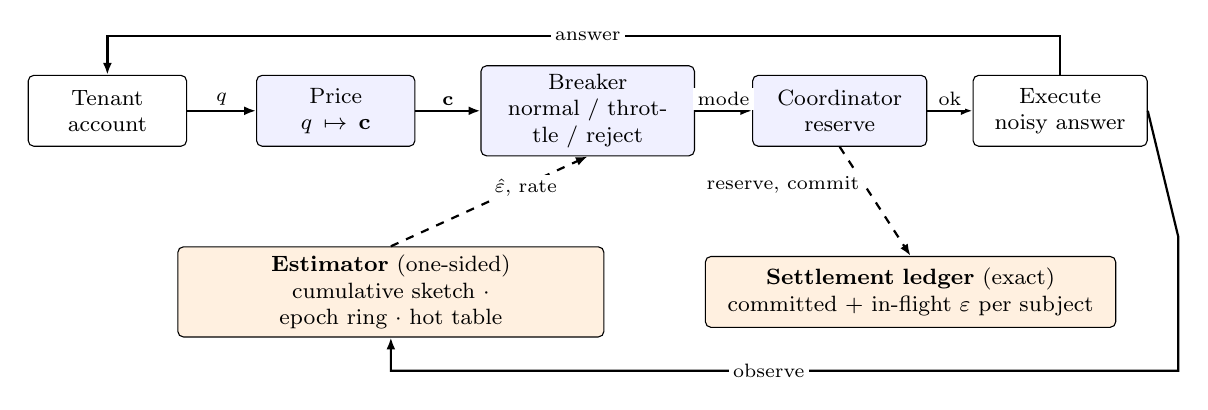
\begin{tikzpicture}[
  font=\footnotesize,
  base/.style={draw, rounded corners=2pt, align=center, minimum height=9mm,
               inner sep=3pt, fill=white},
  ctl/.style={base, fill=blue!6},
  st/.style={base, fill=orange!12},
  ar/.style={-{Latex[length=1.5mm]}, thick},
  lab/.style={font=\scriptsize, inner sep=1.5pt, fill=white},
]
\node[base, text width=1.8cm] (ten)   at (0.0,0)  {Tenant\\account};
\node[ctl,  text width=1.8cm] (price) at (2.9,0)  {Price\\$q\mapsto\cost$};
\node[ctl,  text width=2.5cm] (brk)   at (6.1,0)  {Breaker\\normal / throttle / reject};
\node[ctl,  text width=2.0cm] (coord) at (9.3,0)  {Coordinator\\reserve};
\node[base, text width=2.0cm] (exec)  at (12.1,0) {Execute\\noisy answer};
\node[st, text width=5.2cm] (acc) at (3.6,-2.3)
      {\textbf{Estimator} (one-sided)\\cumulative sketch $\cdot$ epoch ring $\cdot$ hot table};
\node[st, text width=5.0cm] (led) at (10.2,-2.3)
      {\textbf{Settlement ledger} (exact)\\committed $+$ in-flight $\eps$ per subject};

\draw[ar] (ten) -- node[lab,above]{$q$} (price);
\draw[ar] (price) -- node[lab,above]{$\cost$} (brk);
\draw[ar] (brk) -- node[lab,above]{mode} (coord);
\draw[ar] (coord) -- node[lab,above]{ok} (exec);
\draw[ar] (exec.north) -- (12.1,0.95) -- (0.0,0.95) -- (ten.north);
\node[lab] at (6.1,0.95) {answer};
\draw[ar] (exec.east) -- (13.6,-1.6) -- (13.6,-3.3) -- (3.6,-3.3) -- (acc.south);
\node[lab] at (8.4,-3.3) {observe};
\draw[ar, dashed] (coord.south) -- node[lab,left,pos=0.35]{reserve,\ commit} (led.north);
\draw[ar, dashed] (acc.north) -- node[lab,above right]{$\hat{\eps}$, rate} (brk.south);
\end{tikzpicture}
\caption{Request path. Solid arrows carry requests and answers, dashed arrows carry
accounting state. The ledger enforces the cumulative cap exactly; the estimator
supplies windowed and tenant-level pressure and may over-estimate but never
under-estimate.}
\label{fig:arch}
\end{figure*}

\subsection{Pricing a Query}
\label{sec:design-price}

A query plan declares a sensitivity upper bound $\Delta$ and a target
per-query $\eps_q$ at a fixed $\delta$. Under zCDP the platform answers with a
Gaussian mechanism whose scale is $\sigma=\Delta/\sqrt{2\rho_q}$, where $\rho_q$
inverts \eqref{eq:zcdp} at $\eps_q$; a Laplace mechanism is priced with
$\eps_{\mathrm{pure}}=\Delta/b$ and $\rho=0$. The resulting $\cost(q)$ is the unit
of account for every structure that follows, and the inversion is what lets a
tenant ask for ``$\eps_q{=}0.25$ per query'' and receive a price in $\rho$ that
composes without further conversion. Pricing is conservative: the pricer takes an upper bound on sensitivity, because
an under-priced query is an unbounded liability while an over-priced one merely
triggers the breaker early. The controller never re-prices between reservation and
commit, so a crash cannot change the price of an answer already computed.

\subsection{A One-Sided Estimator}
\label{sec:design-accountant}

The estimator keeps three structures. A \emph{cumulative layer} is a pair of
Count-Min sketches, one over $\eps_{\mathrm{pure}}$ and one over $\rho$, so that
mixed pure-DP and zCDP charges compose without conversion on the hot path. An
\emph{epoch ring} is a bounded deque of epochs, each with its own pair of
sketches, supplying the windowed view of \eqref{eq:window}. A \emph{hot table}
holds the $H$ subjects with the largest accumulated charge exactly, because those
are the subjects whose budgets bind.

For key $s$ and cost $c$, the conservative update computes
$m_j=\min_{r} A_j[r,h_{j,r}(s)]$ per layer and raises every cell on $s$'s row
that falls below $m_j+c_j$ to $m_j+c_j$; the estimate is the minimum over rows.
The rule never decreases a cell and never increases an estimate, which is the
property we need. Standard Count-Min with plain increments also over-estimates,
but conservative update keeps the estimate closer to the truth for the same width
by refusing to charge collisions that the minimum already accounts
for~\cite{fusy2022phase,fusy2023countmin}. With $d=\lceil\ln(1/\delta_s)\rceil$
rows and $w=\lceil e/\eps_s\rceil$ columns, the estimate exceeds the true charge
by at most $\eps_s$ times the layer's total mass with probability at least
$1-\delta_s$, and the bound is one-sided: it bounds the excess from above rather
than bracketing an unbiased estimate.

The hot table interacts with the sketch in a way that needs care. An evicted
subject that returns must not restart from zero, because the sketch already holds
its past. We \emph{seed} it with the sketch's current upper bound and then
accumulate exactly. The estimate is therefore the sketch's bound on the past plus
the exact charge since re-admission, which still bounds the true total, with
excess at most the sketch's error at the moment of eviction. Seeding from below,
for instance with the point estimate minus one standard deviation, would restore
accuracy at the cost of soundness, and we do not do it.

The epoch ring is sized so that a window is always covered. With epochs of length
$\ell$ and a ring of $R$ epochs, a window straddling a boundary spans at most
$\lceil W/\ell\rceil+1$ epochs, so we require $R\ge\lceil W/\ell\rceil+1$ and set
the ring size to exactly that bound. An earlier version used
$R=\lceil W/\ell\rceil$, which silently dropped the oldest epoch of every
straddling window and made the windowed estimate an under-estimate by up to one
epoch of traffic. The fix is one line, but it is the difference between a
one-sided estimator and one that is not, and it is the kind of error a purely
cumulative test suite does not catch. Summing per-epoch bounds is itself a bound,
so the ring preserves one-sidedness without further argument.

Total state is $O(dw)$ for the cumulative layer, $O(Rdw)$ for the ring and $O(H)$
for the hot table, none of which depends on $N$. The default uses $w=2^{14}$, $d=4$,
$R=3$ and $H=1024$, occupying 4.7\,MB at $10^6$ subjects and not growing when the
population doubles. The price is an over-estimate that is invisible for heavy
hitters---the hot table holds them exactly---and bounded by $\eps_s$ times the layer
mass for the tail, where the cap is least likely to bind.
Section~\ref{sec:eval-accuracy} measures both effects.Section~\ref{sec:eval-accuracy} measures both
effects.

\subsection{From a Cap to an SLO}
\label{sec:design-slo}

A cumulative cap alone produces the wrong behaviour at both ends: a tenant that
spends a subject's budget in the first hour gets full service for an hour and
nothing thereafter, while one that spreads the same spend over thirty days gets
uniform service. Neither is what the subject agreed to. \sys\ therefore evaluates a population-level SLO:
over a window of length $W$, the fraction of monitored subjects whose spend
exceeds $\theta_{\mathrm{soft}}=\alpha E$ must not exceed $p$, and no subject may
exceed $E$. The default is $\alpha=0.8$, $p=0.01$, $W=600$\,s and $\ell=300$\,s
epochs, so the ring holds three epochs.

The monitor reads the windowed estimates of the hot table rather than of the whole
population, on the argument that a subject outside the hot set has, by construction,
accumulated less than the eviction threshold and cannot be the subject whose spend
violates the soft threshold. This keeps the monitor's cost independent of $N$ and
concentrates attention where violations are possible, but the reported rate is over
the \emph{violation-capable} subpopulation rather than over all subjects. The
tenant-level rate is refreshed every 64 evaluations, bounding staleness at the cost
of a lag between a change in behaviour and the breaker's response.

The breaker is a four-level machine (normal, throttle, reject, freeze) that
escalates immediately and de-escalates one level at a time. De-escalation
requires pressure below the current threshold by a margin $h$ for $d$ consecutive
evaluations: the margin prevents oscillation around a threshold, the dwell prevents
one quiet evaluation from releasing a subject about to be charged again. In throttle
mode the charge is scaled by $\beta=0.5$, which inflates the noise by
$1/\sqrt{\beta}$; the tenant receives a lower-quality answer at a lower price rather
than a refusal. This turns a hard wall into a degradation curve, and it is sound
because the mechanism executed is the one charged for.

\subsection{Two-Phase Settlement}
\label{sec:design-settle}

Reservation is all-or-nothing over the query's subject set. Under a guard covering
exactly the stripes of those subjects, the coordinator reads
$\mathrm{remaining}(s)=E_s-(\text{committed}(s)+\text{in-flight}(s))$ for every
$s$ in the support and rejects if any subject lacks room; otherwise it records a
reservation with a time-to-live. Check and record share the guard, so no other
transaction observes the budget between them, and a rejection is not a partial
charge: either the query is reserved against every subject it touches, or it
touches no budget at all.

Commit is idempotent in the transaction identifier. A repeated commit for an
already-committed transaction increments a duplicate counter and returns the
existing record rather than charging again, which makes client retries safe.
Release returns the reserved budget and is a no-op for a transaction already
committed or released. Reservations neither committed nor released within their
TTL are expired by a periodic tick, bounding the budget a crashed client can hold
hostage to one TTL; the cost is a window in which budget is unavailable although
no answer was delivered, so the TTL trades availability under crash against
availability under load.

Concurrency is handled by striping. Subjects map to $L=64$ stripes by a hash of
the identifier, and a transaction acquires its subjects' stripes in sorted index
order, which rules out deadlock and lets transactions over disjoint subjects
proceed in parallel. A transaction spanning many subjects serialises against everything sharing its
stripes, which is correct for a multi-subject query and is why striped and global
locking behave alike when all traffic hits one subject. The difference appears
when subjects are disjoint, and Section~\ref{sec:eval-concurrency} measures
both.

\section{Analysis}
\label{sec:analysis}

We state the properties the design guarantees and sketch why they hold. The proofs
are short because the mechanisms are chosen to make them short: one-sidedness is an
invariant of an update rule, safety of a check-and-record, atomicity of an
identifier.

\begin{proposition}[One-sidedness]
\label{prop:onesided}
For every subject $s$ and time $t$, the cumulative estimate satisfies
$\hat{\spend}_s(t)\succeq\spend_s(t)$, and the windowed estimate
$\hat{\spend}_s(t,W)$ satisfies $\hat{\spend}_s(t,W)\succeq\spend_s(t,W)$, where
the comparison is componentwise on $(\eps_{\mathrm{pure}},\rho)$.
\end{proposition}

\begin{IEEEproof}
Fix a layer $j$ and let $T_j(x)$ be the true charge of key $x$. We maintain the
invariant that for every key $x$, $\min_r A_j[r,h_{j,r}(x)]\ge T_j(x)$. It holds
initially with all cells zero. On an update of key $x$ by $c$, the conservative
rule sets each cell on $x$'s row to $\max(a,\,m+c)$ where $m\ge T_j(x)$ is the
current row minimum, so every cell on that row becomes at least $T_j(x)+c$, and
cells of other keys only increase. The invariant is preserved. A subject held in
the hot table is seeded with the sketch's bound at re-admission, hence at least
$T_j(x)$ at that instant, and is then incremented exactly, so the invariant holds
there too. The windowed estimate sums whole epochs that cover the window, each
bounded below by its true charge, and charges are non-negative; hence the sum
bounds the true windowed charge.
\end{IEEEproof}

Over-estimation costs availability; Section~\ref{sec:eval-accuracy} measures 0.02\%
relative error for the top percentile and no false negatives in 24 configurations.

\begin{proposition}[Cap safety]
\label{prop:safety}
If every platform reserves through the shared coordinator before executing, then
no admitted transcript produces $\spend_s(t)\succ E_s$ for any subject, even
when tenants split their traffic across accounts and platforms.
\end{proposition}

\begin{IEEEproof}
Let $C_s(t)$ be the committed charge and $F_s(t)$ the reserved-but-uncommitted
charge at time $t$. The coordinator admits only when
$C_s(t)+F_s(t)+\cost(q)\preceq E_s$ for every subject in the support, and the check
and the insertion occur under the same stripe guard, so no transaction interleaves
between them. On commit $F_s$ decreases and $C_s$ increases by the same vector; on
release $F_s$ decreases. Hence $C_s(t)+F_s(t)$ is non-decreasing and bounded by
$E_s$, and the loss actually incurred is bounded by it. Splitting does not
enter the argument because the key of every reservation is the subject, not the
account or the platform.
\end{IEEEproof}

\begin{proposition}[Exactly-once settlement]
\label{prop:atomic}
Under crashes and retries, each admitted query is charged at most once, and no
answer is delivered without a committed charge.
\end{proposition}

\begin{IEEEproof}
Commit is keyed by the transaction identifier and returns the existing record if
the transaction is already committed, so a retry cannot charge twice. The
platform calls commit before returning the answer to the tenant, so an answer
that leaves the platform has a committed charge; a crash before commit means the
answer is never delivered. A reservation that is neither committed nor released
is expired after its TTL, which bounds the budget held by a dead client. The
protocol can therefore over-charge a subject whose answer was computed but lost
to a crash, which is the safe direction, but cannot release data without
charging for it.
\end{IEEEproof}

\begin{proposition}[Bounded instability]
\label{prop:stability}
For a single breaker key, the number of de-escalations in $T$ evaluations is at
most $\lfloor T/d\rfloor$, where $d$ is the dwell parameter.
\end{proposition}

\begin{IEEEproof}
A de-escalation requires $d$ consecutive evaluations below the current
threshold minus the hysteresis margin, and the counter resets on any evaluation
that is not below it. Each de-escalation therefore consumes at least $d$ distinct
evaluations.
\end{IEEEproof}

The bound is loose---E7 observes 12 de-escalations over roughly 5{,}000 evaluations
with $d=3$---but it has the right shape: transitions are controlled by a parameter
rather than by the load, and removing hysteresis raises the count to 26.

Two properties are deliberately absent. We do not prove that estimator error stays
below a constant as the population grows, because the Count-Min guarantee is
relative to total mass; we measure it instead. Nor do we prove that the SLO is met
under every arrival process: the breaker is a feedback controller, and an abrupt
load increase can drive pressure past the reject threshold before it reacts. What
we prove is that the hard cap survives such a transient, because an exact structure
enforces it.

\section{Implementation}
\label{sec:impl}

\sys\ is a reference implementation in Python 3.11: about 5{,}900 lines across 52
modules with 45 tests. The enforcement core depends only on the standard
library; NumPy, pandas and matplotlib are used by the experiment drivers, so the
measured per-request cost is not an artefact of a numerical stack.

Two components are stubs. The ledger backend has an in-memory implementation and
a Hyperledger Fabric adapter that raises \texttt{NotImplementedError}; the
coordinator's safety argument does not depend on the backend, which sees only
reserve, commit and release, but we do not measure Fabric latency, so our numbers bound
the protocol rather than the settlement path. The attester is null: verifying that a platform ran the mechanism it charged for
needs remote attestation or verifiable computation. Coordinator durability is the
backend's, not the protocol's.
Every run is seeded and writes raw rows with metadata, so one command
regenerates every table and figure. An
anonymized artifact with the sources, drivers and raw rows accompanies the
submission.

\section{Evaluation}
\label{sec:eval}

\subsection{Methodology}
\label{sec:eval-method}

We run on a two-vCPU container with 4\,GiB of RAM and CPython 3.11; the host is
deliberately small, so absolute latencies are a conservative upper bound. Experiments
use three seeds and report the mean, except the cap sweep, which is rerun on twelve;
per-seed rows ship with the code.

The generator produces $12{,}000$ requests from $40$ tenants over $1{,}500$
subjects and three platforms, with popularity from a truncated Zipf law of exponent
$1.15$ and $15\%$ of requests touching several subjects; every subject carries a cap
of $\eps{=}1.0$ at $\delta=10^{-5}$. Identities are drawn by inverse transform, so
large ranks fold back onto small ones and the heavy hitters that make accounting hard
survive.
The splitting attack gives an adversary $12$ target subjects, a budget of
$0.30\eps$ per target and $k$ fragments from $12$ to $60$, issued under distinct
identities across platforms.

We compare against five policies: \emph{static quota}, a fixed per-platform
allowance that meters spend but can neither throttle nor window it; \emph{token
bucket}, a per-subject allowance that refills at $0.05\eps$ per second; \emph{audit only}, which admits everything and
flags subjects afterwards and is the deployed status quo; \emph{exact blocking},
per-platform counters checked against composed spend; and \emph{exact global}, exact
per-subject counters shared across tenants and platforms, with no window, breaker or
degradation. \sys\ is the only
policy that is subject-keyed across platforms, time-structured and memory-bounded in
its estimator.

\subsection{Is the Estimator Sound and Accurate?}
\label{sec:eval-accuracy}

A false negative in the estimate cannot release an over-cap answer, because the
ledger refuses it; what an under-estimate costs is a late throttle, which is why
the estimator is built one-sided. Across 24 configurations---four widths, with and
without the hot table, three seeds---the estimate never falls below the true charge,
as Proposition~\ref{prop:onesided} requires, including across eviction and
re-admission.

The monitor, not the estimator, limits what the SLO means (E25). At 24 checkpoints of
a 600\,s trace at cap 0.5 we recompute the exact windowed composition of every subject
and compare it with the rate the hot table reports. In the heavy-tailed population the
table's recall is 1.0 for $H\ge64$ and 0.66--0.95 at $H{=}8$, and the monitored rate matches
the population rate to three decimals. Flatten the popularity
(Zipf 0.6) and shrink the table to eight slots and recall collapses to 0.014: 70 of 71
violations are missed, and the monitored rate reads 0.000 against a population rate of
0.002, because violators are no longer heavy hitters. Scanning the sketch over all $N$
subjects recovers every violation in both regimes with at most two false alarms in
1{,}500 subjects---the loss is sampling, not conservatism---but the scan costs $O(N)$
per epoch. The windowed SLO is therefore best effort over the population; the cap is
not.

Accuracy separates along the population. For the top percentile by spend---the
subjects whose budgets bind---relative error is 4.3\% without a hot table at width 512
and 0.02\% from width 2048 up, where the table rather than the width does the work. For
the tail, mean absolute error falls from 0.071$\eps$ to 0.013 and p99 from 0.37 to 0.10;
width 32{,}768 measures zero error, which is why we do not deploy it.

\subsection{What Does It Cost?}
\label{sec:eval-cost}

The estimator costs 27--32\,$\mu$s per request across widths from $2^{10}$ to
$2^{16}$, against 4.6\,$\mu$s for an exact table: an 18\% rise for a sixteen-fold
increase in width, as expected from eight memory accesses per update plus the hot-table
lookup. The full admission path is slower and far more variable
(Fig.~\ref{fig:latency}a). Its tail came from one function: a tenant-pressure sweep
that scanned the hot table every 64 admissions, which cost p99 5.8\,ms against
0.9\,ms with the sweep removed. We replaced it with an incremental update at commit
time---$O(\text{ring})$ per charge, and a monitor over every charged subject rather
than the hot table---and the p99 falls to 1.1\,ms for the same trace and host, with
the mean moving from 0.28 to 0.23\,ms (E17).

Queueing still decides the deployment (Fig.~\ref{fig:latency}b): at 50\%
utilisation the median is 0.26\,ms but the p99 is 160\,ms; a load that averages
50\% while peaking at five times capacity makes the median 0.9\,s. The path must be
provisioned for its peak, and microsecond averages are the wrong number to quote.

Memory tells the opposite story at small scale: below roughly $10^{4}$ subjects a
dense table is no larger than the sketch, because the sketch's width is paid once and
the table's cost has not caught up (Fig.~\ref{fig:scale}). From $10^{3}$ to $10^{6}$
subjects the dense table grows from 1.2\,MB to 1.2\,GB while the sketch stays at
10.6\,MB (E23); per-request cost rises from 25 to 45\,$\mu$s for the sketch and 9 to
13\,$\mu$s for the table, and the estimate keeps its one-sidedness, with maximum
absolute error 0.057$\eps$ (E8).

\begin{figure}[t]
\centering
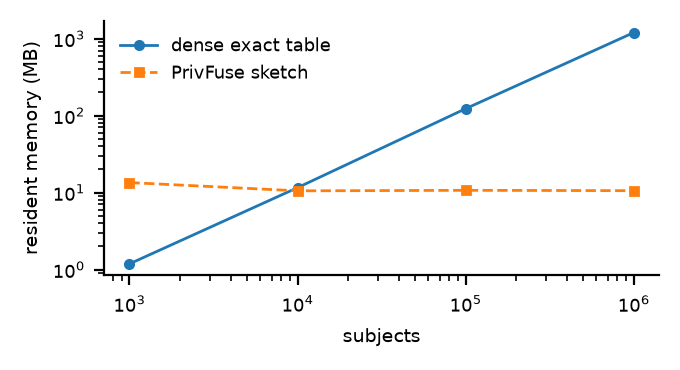
\includegraphics[width=0.88\columnwidth]{figures/fig7_scale.png}
\caption{Resident memory as the subject population grows (E23), with the default
four live tables. The dense table grows linearly with $N$; the sketch is flat. Zero
under-estimates at every population.}
\label{fig:scale}
\end{figure}

\begin{figure}[t]
\centering
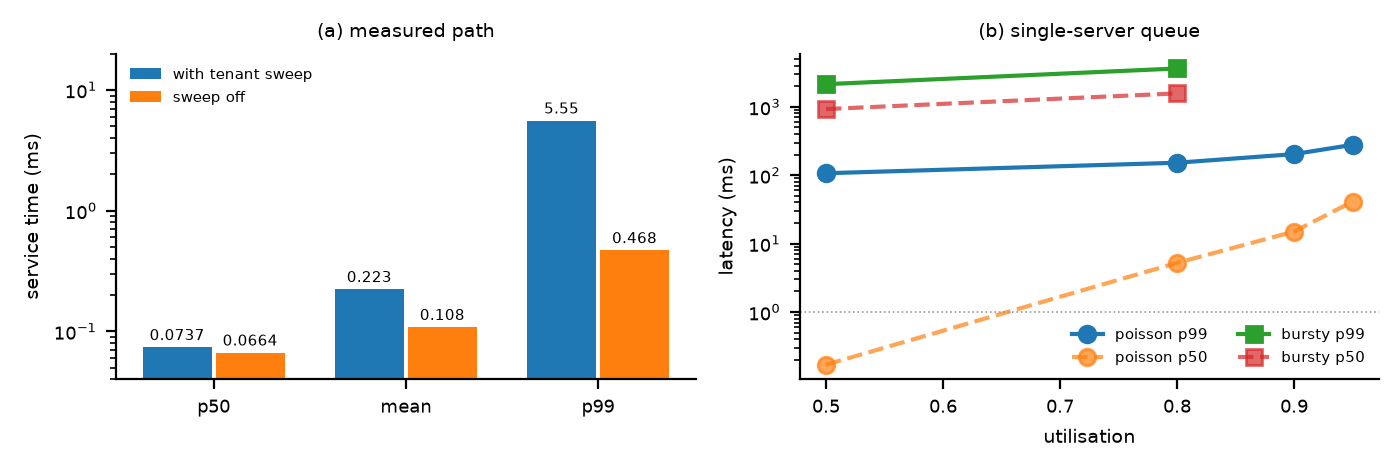
\includegraphics[width=0.9\columnwidth]{figures/fig17_latency.png}
\caption{Admission latency (E17, 12{,}000 requests, median of three trials). (a)
Service time under the per-request pressure sweep and under the incremental monitor we
adopt, log scale. (b) FCFS queue over the measured service times under Poisson arrivals
and under a burst at five times the average rate.}
\label{fig:latency}
\end{figure}


The structure answering windowed queries is therefore $O(1)$ in $N$, whereas a
naive windowed accountant---one cumulative structure per epoch---multiplies the
measured 1.2\,GB by the ring depth. The whole system is not: the ledger keeps one
scalar balance per subject that has ever transacted, far smaller than a cost vector,
and a deployment would shard it.

\subsection{Does Enforcement Hold?}
\label{sec:eval-enforce}

Table~\ref{tab:enforce} reports the central comparison at six cap levels, each
averaged over twelve seeds. At a cap of $\eps{=}1.0$, \sys\ admits 0.934 of requests
and produces no hard-cap violation, while exact per-platform blocking admits 0.978 and
lets 12.7 subjects exceed the cap on average, the worst of them reaching $1.69\eps$.
Static quota behaves similarly at 0.956 availability and the same violation count.
Their counters are exact; the violations come from the key: each platform meters
its own share, so a subject with records everywhere is charged once per platform and
accumulates up to three times the cap, and natural traffic alone pushes a dozen
subjects past it.

An adversary that sees the decision can re-plan (E18): halving a fragment after each
refusal raises \sys's composed loss from 0.80 to 0.85 of the cap, still inside the
hard cap, but raises static quota from 1.30 to 1.74 and exact blocking from 1.69 to
1.76. A smaller request is cheaper and slips under a quota that refused the full
fragment; a keyed account still charges it. Spreading attempts over forty tenants changes
nothing---identity is not the key---but spreading them over three platforms pays,
because each meters its own counter.

The availability gap is the price of soundness and it shrinks as the cap loosens:
13.6 points at $0.5\eps$, 4.4 at $1.0\eps$, 3.4 at $1.5\eps$ and nothing at
$2.0\eps$, where the soft threshold stops binding and \sys\ behaves like exact global
accounting while the baselines still violate the cap twelve times per run. The
$3.0\eps$ cap is a control: no policy violates it, since the trace's maximum is
$2.01\eps$.

\begin{table}[t]
\centering
\caption{Enforcement across cap levels (E15, mean of twelve seeds). ``Viol.'' is
the number of subjects whose cumulative spend exceeded the cap; availability is
the admitted fraction. The 95\% confidence interval of \sys's availability is at
most $\pm0.008$ at every cap.}
\label{tab:enforce}
\footnotesize
\setlength{\tabcolsep}{3pt}
\begin{tabular}{@{}lcccccc@{}}
\toprule
& \multicolumn{2}{c}{\sys} & \multicolumn{2}{c}{Exact blocking} & \multicolumn{2}{c}{Static quota} \\
\cmidrule(lr){2-3}\cmidrule(lr){4-5}\cmidrule(lr){6-7}
Cap & Avail. & Viol. & Avail. & Viol. & Avail. & Viol. \\
\midrule
0.50 & 0.752 & 0 & 0.888 & 15.2 & 0.903 & 15.1 \\
0.75 & 0.854 & 0 & 0.956 & 13.0 & 0.939 & 13.0 \\
1.00 & 0.934 & 0 & 0.978 & 12.7 & 0.956 & 12.7 \\
1.50 & 0.966 & 0 & 1.000 & 12.0 & 1.000 & 12.0 \\
2.00 & 1.000 & 0 & 1.000 & 12.0 & 1.000 & 12.0 \\
3.00 & 1.000 & 0 & 1.000 & 0.0 & 1.000 & 0.0 \\
\bottomrule
\end{tabular}
\end{table}

At $1.0\eps$ \sys\ admits $4.4\pm0.2$ points fewer requests than exact blocking and
$2.2\pm0.2$ fewer than static quota, while both exceed the cap $12.7\pm0.3$ times per run
against zero; the paired difference is tighter than the interval because every policy
sees the same traces, and deterministic accounting means only the violation count varies
across seeds. Zero violations is an observation over twelve traces, not a proof;
Proposition~\ref{prop:safety} is the proof.

The adversary splits a fixed budget across $k$ identities (E4). The escape ratio of
audit-only and token-bucket policies rises linearly with $k$, from 1.07 at $k{=}12$ to
2.43 at $k{=}60$: audit-only has no key, and the bucket refills $180\eps$ over the
one-hour trace against a $0.3\eps$ fragment, so it never binds. Static quota saturates
at 1.30 and exact blocking reaches 1.69; neither grows with $k$ once the split exceeds
what the per-platform counters absorb.
\sys\ is flat at 0.82 across the range and exact global is flat at 0.98, because
neither can be made to forget that the fragments concern the same subject. The
flatness, not the level, is the result: the attack's only lever is the identity it
uses, and identity is not part of the key.

Exact global is the strongest baseline and it is sound: at $k{=}42$ it admits 0.929
against 0.923 and leaves 2\% of the cap unused against 18\%. The 18\% is the residue
of the soft threshold---\sys\ throttles from $0.8E$ and throttled queries consume half
a charge---so the worst subject ends below its cap rather than at it. What exact global
lacks is a window, a degradation path and an estimator whose memory does not grow with
$N$: the split result shows that subject keying is necessary and that \sys\ achieves
it, not that \sys\ dominates exact global on every axis.


\subsection{Where Is the SLO Frontier?}
\label{sec:eval-slo}

Sweeping the soft threshold $\alpha$ from 0.55 to 0.95 at four values of $p$ moves
availability from 0.749 to 0.794 and raises the fraction of settings at which the SLO
is satisfied from 0.25 to 1.0, while the hard cap never moves: zero violations
everywhere (Fig.~\ref{fig:slo}). The knobs are not independent. At $\alpha{=}0.55$ the
monitored violation rate is 2.2\%, so the SLO holds only for $p\ge5\%$; at
$\alpha\ge0.85$ it is at most 0.22\% and the default $p{=}1\%$ holds. Operators choose
a tight target with a loose rate or the reverse, 4.5 points apart, not both: a small
set of subjects crosses any threshold near zero whatever the policy.

\begin{figure}[tb]
\centering
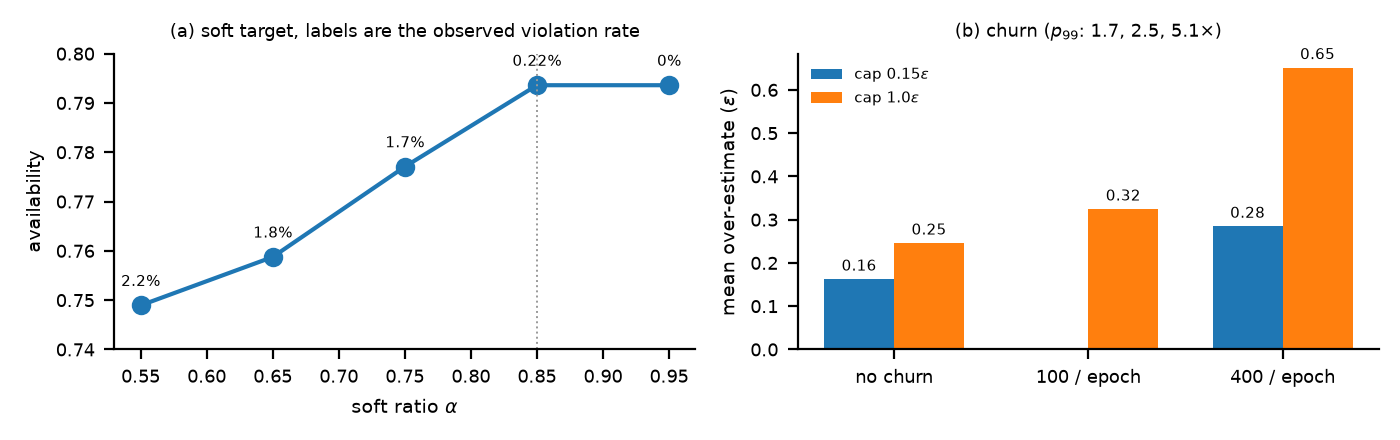
\includegraphics[width=\columnwidth]{figures/fig11_slo_churn.png}
\caption{Operating points. (a) Availability against the soft ratio, labelled with the
observed soft-violation rate; the dotted line is where the default $p{=}1\%$ starts to
hold. (b) Mean over-estimate (E14) when cohorts of heavy subjects are rotated into
the population each epoch (the $0.15\eps$ cap has no 100-cohort run); the hot table
keeps its accuracy only while churn is slow.}
\label{fig:slo}
\end{figure}

The sensitivity sweep varies one factor at a time around the default and uses a
single seed per point, so it locates trends rather than estimating their
variability. Two points bracket aggregation: with one platform, static quota becomes
sound---worst spend $0.969\eps$---because a per-tenant quota on the only platform is
also a per-subject quota; with six, its worst spend rises to $1.859\eps$ while \sys\
stays at $0.825\eps$.
A heavier tail ($\alpha_{\mathrm{zipf}}{=}1.5$) costs 15 points of availability,
from 0.936 to 0.783; 200 tenants cost 4; a 64-entry hot table costs 2; moving
$\delta$ from $10^{-6}$ to $10^{-4}$ raises availability from 0.920 to 0.941; and
crashes at 0.05 cost one point. Across all 19 points violations are zero and the
estimator never under-estimates.

\subsection{Ablation and Stability}
\label{sec:eval-ablation}

Removing one component at a time (three seeds, E7) gives the following. The full
system admits 0.923 of requests at 4.77\,MB and 100.9\,$\mu$s per request; exact
global admits 0.929 at 0.24\,MB and 10.8\,$\mu$s. Removing degradation, so that the
breaker can only admit or refuse, costs 4.2 points of availability (0.881 against
0.923): degradation converts would-be refusals into answers. Shrinking the sketch from $2^{14}$ to $2^{9}$ columns cuts memory from 4.77\,MB to
0.71\,MB without moving availability, and widening it to $2^{16}$ only costs memory:
on 1{,}500 subjects the hot table holds everyone who matters.

Churn is the cost the capacity sweep hides (E14, Fig.~\ref{fig:slo}b): rotating 400
new heavy subjects per epoch raises the mean over-estimate from 0.16 to 0.28 at a
$0.15\eps$ cap and from 0.25 to 0.65 at $1.0\eps$, and the p99 from 1.7$\times$ to
5.1$\times$. Safety is untouched---zero violations in 30 runs---because an evicted
subject is re-seeded from the sketch upper bound, but the table stops paying for
itself, which bounds what it can buy against an adversary who chooses the traffic.

The hot-table row is a warning. Disabling the table raises availability from
0.923 to 0.930 and lowers cost from 101 to 80\,$\mu$s, but the breaker's flap count
falls to zero: the monitor samples its violation rate from the hot table, so a
capacity of one blinds the SLO machinery. Ablating the table silently ablates the
monitor.



The last row is the honest comparison, and it is less comfortable than it
suggests. At 1{,}500 subjects exact cumulative accounting matches \sys's
availability within a point ($0.898$ against $0.906$ at $1.0\eps$; $0.713$ against
$0.721$ at $0.5\eps$) with 0.38\,MB against 5.0\,MB. Its 19\,$\mu$s per request is not
a like-for-like cost: it runs no breaker, coordinator or window. A windowed exact accountant is likewise implementable (E16, 600\,s window): at
$0.5\eps$ it admits every request and still lets six of 1{,}500 subjects exceed their
\emph{lifetime} cap, spending 1.08\,MB against \sys's 5.0\,MB. Windowed enforcement
bounds a window, not a lifetime, and at $1.0\eps$ the two are within a point of
availability ($1.000$ against $0.906$) with one lifetime violation. \sys's case
therefore rests neither on windows being inexpressible nor on exact tabulation being
slow at $10^{3}$ subjects, but on $10^{6}$, where the table is 265\,MB.

On a load oscillating around the threshold, hysteresis and dwell give the breaker
zero transitions, and without them 26, 13 of them reversals.

\subsection{Why zCDP and Not R\'enyi DP}
\label{sec:eval-backend}

The choice of algebra is usually about tightness; for admission it is about
solvability. A R\'enyi accountant evaluates a discrete grid of orders and converts to
$(\eps,\delta)$, and that conversion floors at $\log(1/\delta)/(\alpha_{\max}-1)$,
which for $\delta=10^{-5}$ and $\alpha_{\max}=512$ is $0.0225$. A tenant asking for
$\eps_q{=}0.02$ sits below the floor, so no scale on this grid certifies it: our
implementation saturates at $\sigma=1000$, 4.17 times the zCDP scale, and reports
$\eps{=}0.023$ with \texttt{reached\_target} false rather than accepting the query.
Basic composition needs $\sigma=240$ for the same target but reports $0.2008$ after
100 charges, ten times zCDP's budget. At $\eps_q{=}0.1$ the three backends agree to
within 0.004\% in $\sigma$ and in composed $\eps$ (1.0195 against 1.0194), and at
$0.5$ to within 0.006\%. The conclusion is narrow: zCDP is the only backend that both
calibrates the mechanism and composes it without discarding an order of magnitude;
R\'enyi DP remains right for training-time accounting at larger budgets.

\subsection{What Soundness Costs in Utility}
\label{sec:eval-utility}

The utility experiment spends a subject's whole budget on counting queries over one
predicate and measures the $F_1$ of each answer against the truth. At
$\eps_q{=}1.0$ \sys\ answers one query at 0.823, against 0.900 for an unbounded
policy that answers 100 queries for 100$\eps$; at $0.5\eps$ two queries at 0.552
against 0.881; at $0.25\eps$ four at 0.542 against 0.871, and both baselines exceed
the cap in every seed, so their accuracy is bought with a violation. The gap at small
$\eps_q$ is the budget, not overhead: four noisy answers cannot match a hundred.
Degradation costs less: 699 of 5{,}088 admitted queries are throttled, 13.7\%, worth
the 4.2 points of availability measured in the ablation.

\subsection{Settlement and Concurrency}
\label{sec:eval-concurrency}

Five settlement invariants pass, including the refusal to re-bind a reserve;
Table~\ref{tab:faults} reports the crash points. In the atomicity test, 16 threads issue 3{,}200
attempts against a subject whose cap funds exactly 100 charges; every thread count from
2 to 16 admits exactly 100, spends exactly $1.0\eps$, and records zero violations.

Injecting a crash at each step of the transaction tests
Proposition~\ref{prop:atomic} directly (Table~\ref{tab:faults}, E19), with the
invariants read off the ledger rather than off the caller's bookkeeping. Over every
crash point, one and four threads, and a crash rate up to 5\%, no answer left without
a committed charge, no transaction was charged twice, and in-flight spend never
crossed the cap; the price is the crash rate itself, 188 of 200 requests delivered at
5\%, plus one request in 800 blocked by a suspended hold. Three platforms with one
ledger each, the last row, are the control that motivates the shared coordinator.

\begin{table}[tb]
\centering
\caption{Fault injection at each settlement step (E19): one subject, cap
$1.0\eps$, unit $0.05\eps$, five-second TTL, retry with the same id. A row is sound
when answers never exceed commits.}
\label{tab:faults}
\footnotesize
\setlength{\tabcolsep}{3pt}
\begin{tabular}{@{}llrrl@{}}
\toprule
Crash point & Retry & Ans. & Com. & Outcome \\
\midrule
none                        & ---       & 1 & 1 & delivered \\
reserve or execute          & same id   & 1 & 1 & charged once \\
reserve or execute          & after TTL & 0 & 0 & hold returned \\
commit                      & any       & 0 & 1 & answer withheld \\
\midrule
per-platform ledgers        & ---       & 60 & 60 & $3.0\times$ cap \\
\bottomrule
\end{tabular}
\end{table}

Throughput depends on the workload, and our earlier reading was too pessimistic. With
every thread contending for one subject, striping buys nothing: four threads reach
21.4k reserve-and-commit operations per second against 26.5k for a single global lock,
and even one thread is 28\% slower. With disjoint subjects the same code scales: four
threads reach 91.5k against 25.2k, a factor of 3.6, because a transaction waits only
for the stripes it touches (E13, medians of three). Striping removes a serialisation
point, not contention: concentrated traffic will not benefit.

Served over loopback, one client sustains 1.9k pairs per second at a 201\,$\mu$s
median round trip and four sustain 2.4k at 283\,$\mu$s, p99 16\,ms; the server
saturates, so more needs sharding. Three caveats: one process, a loopback trip, and a
stub ledger adapter that hides a real commit trip.

\section{Related Work}
\label{sec:related}

\emph{Privacy accounting.} Recent work on continual observation separates
oblivious from adaptive adversaries~\cite{bun2026separating} and revisits the cost
of answering online queries~\cite{bun2016make}. Tight auditing has become its own
line, from reconstruction attacks on production query systems~\cite{cohen2018linear}
to Gaussian-DP audits of synthetic data generators~\cite{ganev2026tight} and
analyses of the gap between provable and auditable privacy in
DP-SGD~\cite{modi2026revisiting}. All of it asks how large the loss was; \sys\ asks whether the next release may
happen. We do not improve a composition bound: we take
zCDP~\cite{bun2016concentrated} and make it cheap and monotone enough for an
admission path, and measure R\'enyi~\cite{mironov2017renyi} and Gaussian
DP~\cite{dong2021rejoinder} against it for that purpose.

\emph{Systems that enforce privacy.} PINQ established the pattern of a query
interface that charges a budget per analyst~\cite{ebadi2015featherweight}; Fuzzi and
Flex turn it into a deployed SQL system with elastic sensitivity and per-query
pricing~\cite{johnson2018towards}, and production libraries apply the same
accountant to training~\cite{yousefpour2021opacus,abadi2016deep}. All three fix the accounting unit to the analyst and settle inside one
administrative domain. Cohere tracks DP budgets for large-scale analytics pipelines at block
granularity~\cite{kchler2024cohere}; PrivateKube schedules one budget across
competing tenants~\cite{luo2021privacy} and DProvDB tracks provenance across
colluding analysts~\cite{zhang2023dprovdb}. All three key the budget to an analyst,
an application or a block inside one deployment, so none charges a subject whose
records sit on several platforms. Prochlo moves enforcement into an enclave and removes the trusted server, fixing the
unit to the user and the granularity to a batch~\cite{bittau2017prochlo}, a model now
studied formally as anonymous shuffling~\cite{cheu2019distributed}; IncShrink
combines MPC with DP at a cryptographic protocol per query~\cite{wang2022incshrink}. None of them charges a \emph{subject}
whose records sit on several platforms, and none treats the resulting counter as a
transaction.

\emph{Auditing and governance.} A parallel literature builds the machinery for
post-market monitoring~\cite{mokander2021conformity} and ethics-based
audit~\cite{mokander2021ethicsbased}, and empirical studies show how far declared
policy is from measured behaviour~\cite{kapp2024collection}. Recent work
extends governance to AI-mediated platforms~\cite{shouli2025ethical}. \sys\ assumes
the declaration exists and makes it enforceable at the point of sale.

\emph{Data markets.} Trustless trading has occupied the blockchain systems
community, with recent designs scaling delivery and
settlement~\cite{liu2025yotta} and provenance mechanisms tracking derived
artifacts~\cite{zhu2025auditing}. These answer ``did I receive what I paid for?''. Pricing privacy has been studied as
a negotiation between subject and buyer~\cite{jung2019privacy}, presupposing a budget
that can be spent and tracked; the prior question---``may this answer be sold at
all?''---is orthogonal, and the ledger records payments, not budgets. We keep the ledger as the settlement substrate and add a
budget root that every platform consults; we are not aware of prior work that makes
the charge itself a two-phase transaction keyed by the subject across platforms.

\emph{Approximate counting.} Count-Min sketches and their conservative variants are
well understood~\cite{fusy2023countmin,fusy2022phase}, including on power-law
streams, and learned variants reduce error at the same width~\cite{nishishita2025optimized}.
We want not the smallest error but an error with a known sign, which rules out
unbiased estimators and makes conservative update the right primitive.

\emph{Mechanisms.} Every mechanism we price exposes a cost
vector: DP synthesis~\cite{saha2024dpcda}, spectral
perturbation~\cite{feng2023spectraldp}, geometric
preconditioning~\cite{bosch2026dpkfc,duan2025technical}. How the vector is produced
changes the vector, not the enforcement layer.

\section{Discussion}
\label{sec:discussion}

Three principles transfer. Split the accounting state by the question it answers:
exact where the quantity is money and must be settled, one-sided where it has time
structure and must be cheap. Key every charge on the party that bears the loss, not
the one who pays. Treat the charge as a transaction with a commit point.

A deployment would replicate the coordinator over consensus nodes, own each subject
on one node so the critical section stays local, and shard by subject range; E22 takes
the first step with separate processes on one host. A subject's budget would then live
on one node, which could under-report a charge, and receipts make that detectable only
afterwards; closing it needs Byzantine agreement or a proof that the charge matches
the mechanism executed.

The accounting layer is itself sensitive: the ledger records which subjects appear
in which queries and the hot table is close to a list of the most-queried subjects, so
a reader learns participation patterns without learning any answer. Accumulators,
oblivious access or an enclave each cost something the design does not budget for;
this is the most important open problem here.

Three further limitations bound the claims. The SLO monitor samples the hot table, so
its coverage depends on the hot capacity, and sampling the epoch ring directly is a fix
we have not evaluated. Two adversaries are measured: one that observes throttling and
re-times its fragments (E18, loss 0.80 to 0.85 of the cap, because the key still binds
it) and one that cycles subjects through the hot table (E14, costing accuracy and
availability but never soundness).

Two conditions would falsify the approach. If a population is small and its policy
cumulative, exact counting is cheaper (our ablation, $1{,}500$ subjects); with one
platform a subject-keyed quota is sound, a tenant-keyed one is not. And if a query's
cost cannot be predicted before execution, admission must price conservatively or fall
back to post-hoc charging, weakening the guarantee to the one auditing provides. The
design is for what remains: many subjects, several platforms, many tenants, and a
promise that holds before the answer leaves the building.

\section{Conclusion}
\label{sec:conclusion}

Privacy budgets in data markets are enforced after the fact, keyed on the party that pays
and reconciled outside the transaction that spends them, so a tenant can split its traffic,
release before the overspend is known, and lose the charge on a crash. \sys\ moves the decision to admission around three commitments---an exact
ledger, a one-sided sketch, and a two-phase reservation that separates a budget from a
guess. On a million subjects the estimator holds 10.6\,MB where exact accounting needs
1.2\,GB; enforcement admits 0.93 of requests at $1.0\eps$ with no violations where
per-platform blocking admits 0.98 and breaches the cap a dozen times; and the escape
ratio under a splitting tenant stays at 0.82 where policies without a subject key reach
2.43. The cost, 4.4 points of availability, is reported with the gains.
Next comes privatising the accounting state and replacing trust in one coordinator with
a proof that the charge matches the mechanism that ran.
\enlargethispage{3\baselineskip}


\bibliographystyle{IEEEtran}
\bibliography{refs}

\end{document}